\documentclass[12pt,a4paper]{article}
\usepackage{graphicx}
\usepackage{amsmath}

\textwidth 16cm
\textheight 23.3cm
\topmargin  -2.5cm
\oddsidemargin 0.0cm
\evensidemargin 0.0cm
%\pagestyle{empty}

\renewcommand{\arraystretch}{1.05}

\setlength\unitlength{1mm}

\begin{document}

\title{Static iterations in 3D code -- speed and (in-)stability}
\author{Discussion file: QDD project}
\date{15. May 2019}
\maketitle

The static iteration in the triaxial cluster code ``QDD'' is based on
accelerated gradient iteration. To speed up, one can invoke an
occasional exact diagonalization of the actual mean-field Hamiltonian.
The modulus for this action is the parameter {\tt ifhamdiag}. 
It is supposed to improve convergence if the pool of s.p. states
contains also a couple of unoccupied states. 
 In the
nuclear 3D code, this strategy works so efficiently that one uses {\tt
  ifhamdiag}=1 as standard. This turns out to be nod the case for
molecules/clusters. The problem is analyzed here using the test case
of Na$_8$ and Na$_{12}$ with ionic background.

\medskip

\centerline{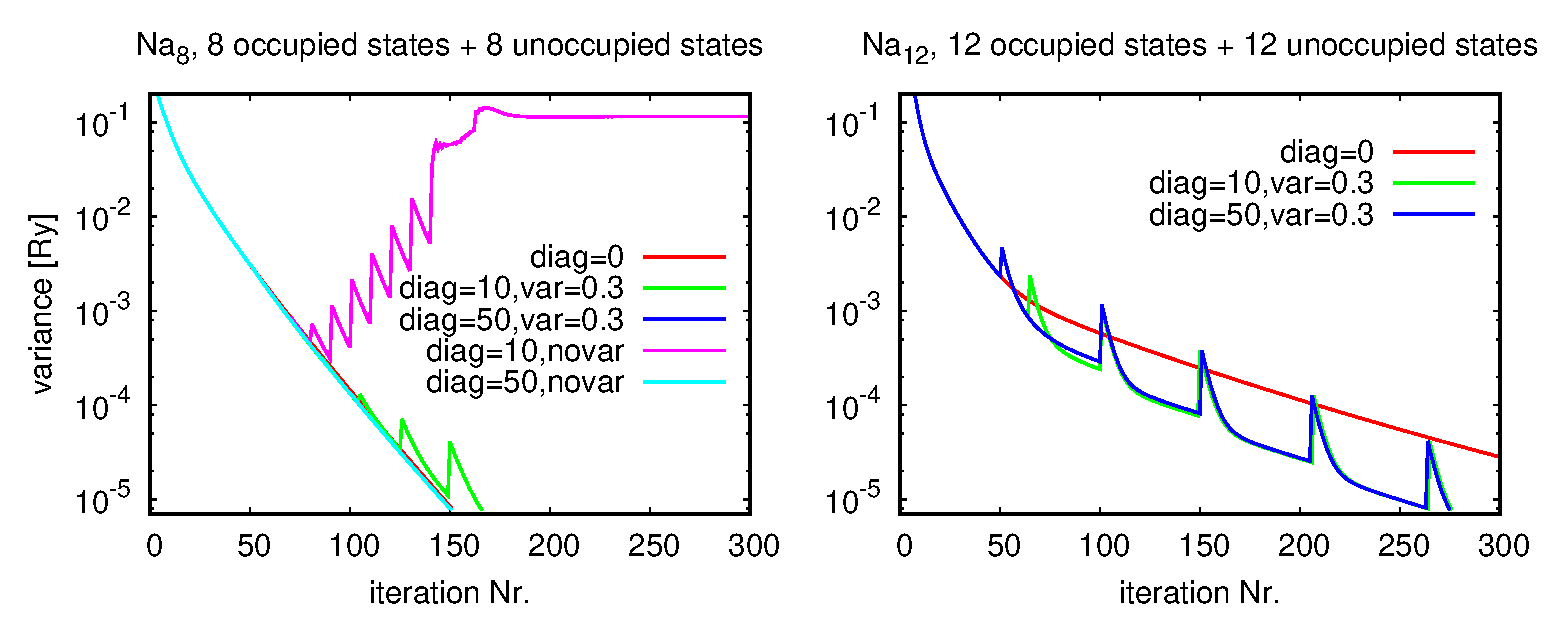
\includegraphics[width=\linewidth]{test_hamdiag.pdf}}

\medskip

The above figure shows the evolution of total variance (r.m.s. average
of s.p. variances) with iterations. We look first at the left panel,
showing results from Na$_8$.  The parameter {\tt ifhamdiag} is
abbreviated by the label ``diag''. The parameter ``(no)var'' stands
for a stabilizing criterion explained below. At the moment, we
concentrate on ``novar'' which means that diagonalization is done
strictly at every ``diag'' iteration.  Reference is the case
``diag=0'' which is straightforward damped gradient iteration without
diagonalization steps.  It converges steadily and fast. Switching to
very occasional diagonalization with ``diag=50,novar'' improves a tiny
bit. Calling for more diagonalization with ``diag=10,novar'' destroys
convergence completely. The hindrance is the interplay with the update
of mean field. Diagonalization in the subspace changes the mean field
suddenly. Even if that may be only a little, the perturbation has not
calmed down sufficiently before the next diagonalization step such
that perturbations accumulate.

The solution is, of course, to choose the proper distance between
diagonalizations. However, this distance depends on the system and it
is asking to much from a standard user to fiddle around with {\tt
  ifhamdiag}. The idea is to let the system check how far recovery
from perturbation went. To this end, we introduce a new input
parameter {\tt variance\_gain} which is the factor about which the
variance has to shrink since the last diagonalization before a
next diagonalization can become effective. The criterion for 
a new diagonalization step is then set by two measures,
first, {\tt ifhamdiag} gradient steps have to done, and second
the actual variance must fulfill
\begin{equation}
  \mbox{\tt variance}
  <
  \mbox{\tt variance\_gain}*\mbox{\tt variance\_old}
\end{equation}
where {\tt variance\_old} is the variance at the last iteration step
before previous diagonalization. The figure above abbreviates var={\tt
  variance\_gain}. A factor of about 1/3 was found to be efficient.
The figure above shows two cases with ``var=0.3'' and both finally
converge well. Still, we see for ``diag=10'' that the turmoil
generated by too often diagonalization causes slight delays in the late
phase.

One may wonder why to bother about diagonalization if straightforward
damped gradient iteration works so well. The answer is given in the
right panel of the above figure which shows results from Na$_{12}$.
Opposed to Na$_8$ which is a magic cluster, this cluster represents an
open shell situation with high level density at the Fermi energy.  It
is obvious that occasional diagonalization delivers significantly
faster convergence even if the diagonalizations spoil for a moment the
variance.

Thus far, we could be happy. An  unpleasant surprise comes if we
chose a situation with fewer unoccupied states. This is demonstrated
in the figure below.


\bigskip

\centerline{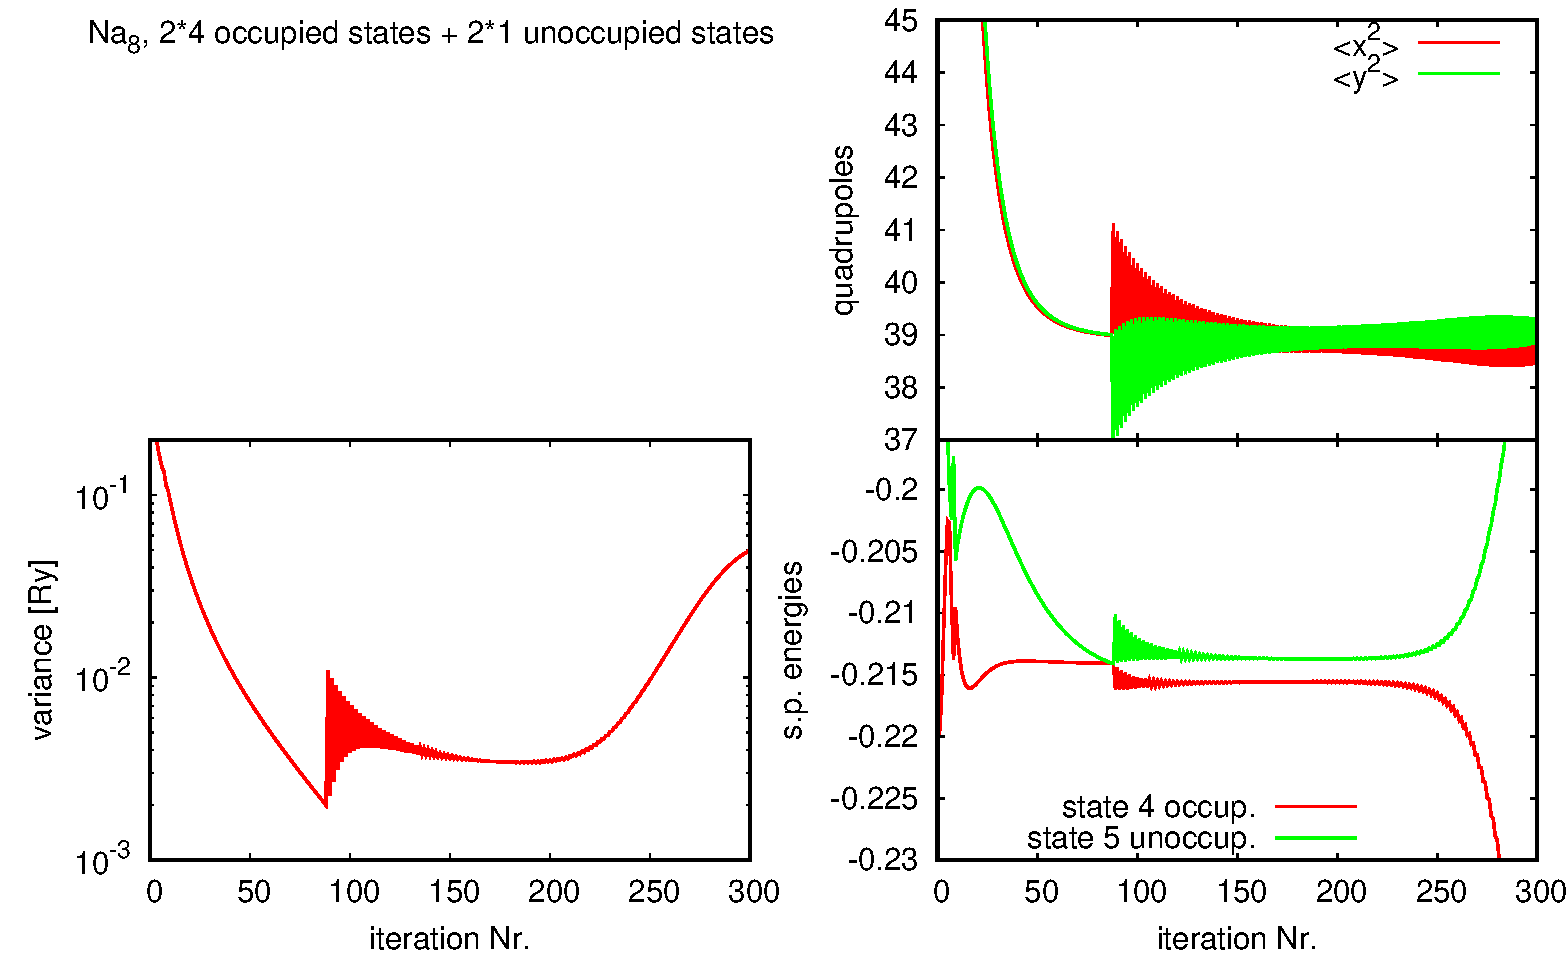
\includegraphics[width=\linewidth]{unstable_iteration.pdf}}

\medskip

It deals with the ``magic'' Na$_8$ and only 1 extra state above the
Fermi energy (in fact, 2 states but spin degenerated) and it uses only
the straightforward damped gradient iteration.  The effect is
dramatic.  At some iteration, the variance (left panel) jumps and
never recovers. The lower right panel shows that the instability
occurs at the very moment where HOMO and LUMO cross.  What then
happens is that these two states exchange their properties from one
step to the next as can be seen from the fluctuations quadrupole
moments (upper right panel). Such a flip-flop iteration is known from
molecules with degenerate ground states. It is a surprise in the
present case where we know that a closed-shell ground state exists.
Even occasional diagonalization cannot cure that dilemma. It seems
that the flip-flop iteration hinders the system from going downhill
into the minimum.  It is likely that the same mechanism is causing the
perturbations in the successful cases discussed first. The larger space
of unoccupied states softens the problem. Still, there is something
to be understood and/or improved.

\end{document}
